\documentclass[12pt]{article}
\usepackage{graphicx}
\usepackage{todonotes}
\usepackage{wrapfig}
\usepackage{lscape}
\usepackage{rotating}
\usepackage{epstopdf}


\usepackage[utf8]{inputenc}
\usepackage{titlesec}
\usepackage{tabu}
\usepackage{multirow}

\setcounter{secnumdepth}{4}

\titleformat{\paragraph}
{\normalfont\normalsize\bfseries}{\theparagraph}{1em}{}
\titlespacing*{\paragraph}
{0pt}{3.25ex plus 1ex minus .2ex}{1.5ex plus .2ex}

\begin{document}
\begin{titlepage}
\begin{figure}[h!]
\includegraphics[width=\linewidth]{Diagrams/kumladi.PNG}
\end{figure}

\begin{center}

\includegraphics[scale=1]{Diagrams/up.jpg}
\begin{huge}
	
\bigskip
\bigskip
\bigskip
\textbf{Buzz}
\bigskip
\bigskip
\bigskip
\end{huge}

 \begin{huge}
 \textbf{Requirements and Design Specifications}
\end{huge}
\newpage
\pagebreak


Compiled By \\[\baselineskip]
{\large

Nkosinathi Mothoa - u12077420\\
Nkosenhle Ncube - u13247914\\
Nathan Ngobale - u15110045\\
Kamogelo Tsipa - u13010931\\
\par}

\end{center}

\end{titlepage}

\newpage
\tableofcontents

\newpage
\section{Vision and Scope}    

\subsection{Project Vision} 

\par{The platform is a discussion forum and is aimed at providing a space where users can collaborate on topics of interest. Users can pose questions on a said topic to the community. Through collaboration the quality of questions and answers on the platform will improve and as a result the user benefits from the community and is able to help others. An example of an instance of the platform would be the use of the platform in the field of education where students/learners use this platform to collaborate and seek help on topics that they might be interested in. To promote collaboration and continued interest, features of gamification will be added to the platform in effort to encourage users to contribute and participate in forum activities.}

\subsection{Project Scope}
\par{The platform is at its core a discussion forum, the selling point of the platform is the use of features of gamification to encourage user participation and contribution. Users will be able to interact with other users activity by commenting on their posts, voting posts up/down, and subscribing to posts to receive notifications on activity related to those specific posts and rewards will be accordingly given for participation.}

\begin{figure}[h!]
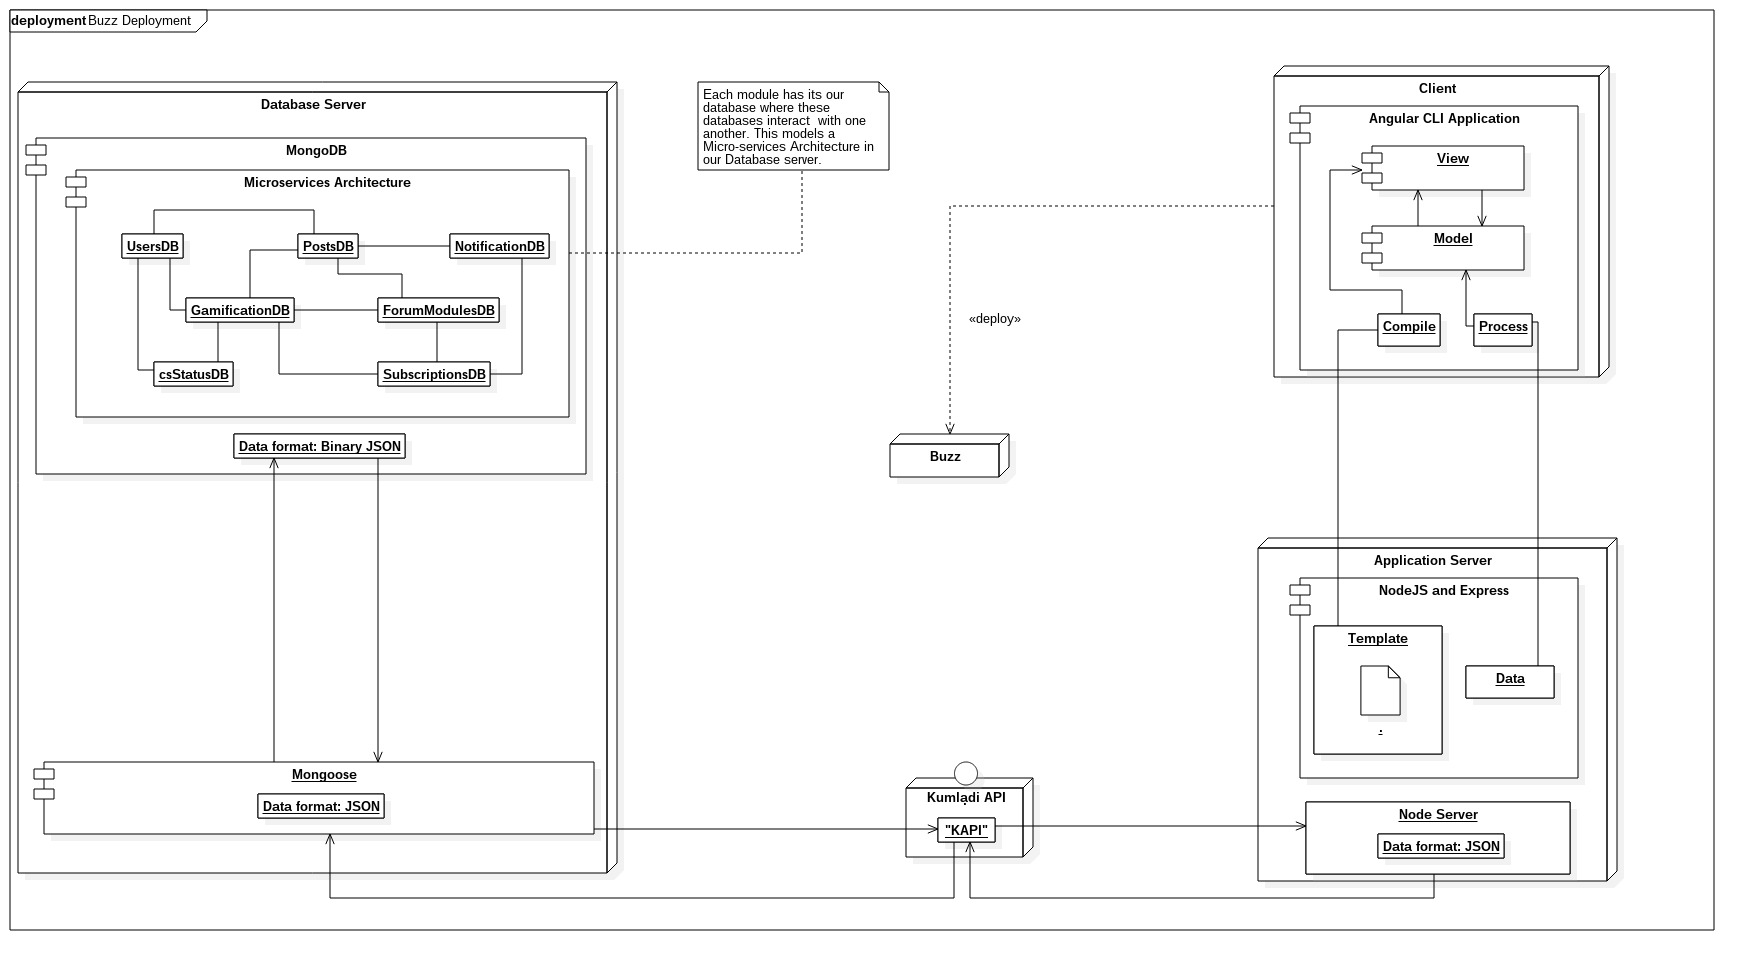
\includegraphics[width=\linewidth]{Diagrams/Deployment.jpg}
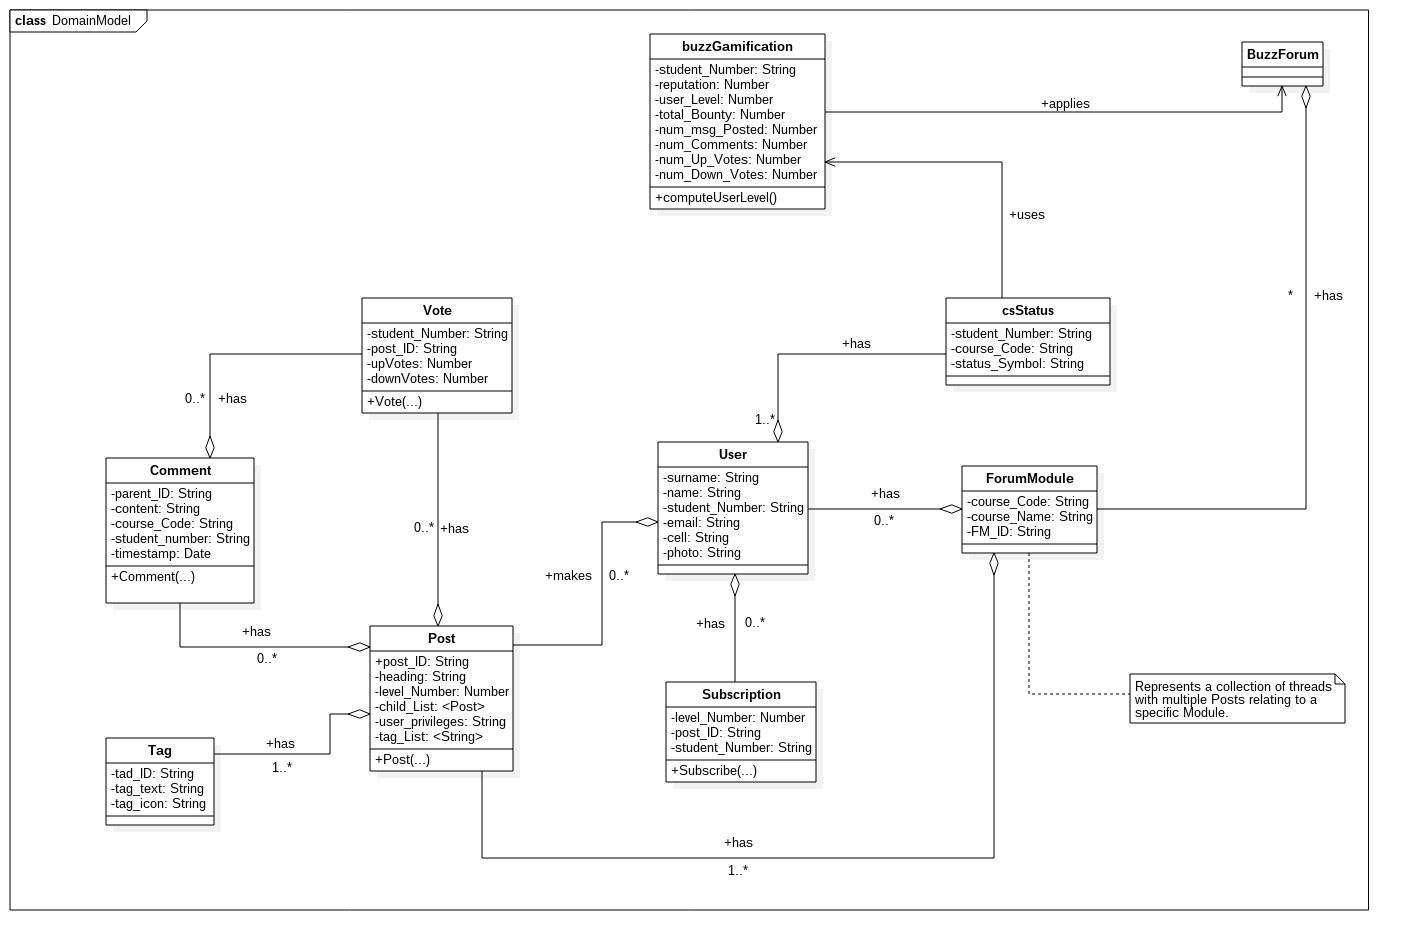
\includegraphics[width=\linewidth]{Diagrams/Domain.jpg}
\caption{Deployment diagram and domain model.}
\label{Use-case: Users Module}
\end{figure}

\newpage 
\subsection{Architecture Design of the System}
\par{At the highest level of granularity the system is based on Service Oriented Architecture(SOA). Second  level of granularity can be visualized as to be based on model-view controller (MVC), which further transcends to micro services in relation to SOA. We apply Model-View-Controller across our Application-Server and Client-application and the Micro-services architecture is applied within our database server (complimented by the Blackboard pattern for inter-connectedness between independent databases).}

\subsubsection{Architecture Design}
\begin{itemize}
\item Service oriented architecture patterns (Micro services) on the database server.
\item The Blackboard pattern, is applied across the application server and client with our Micro-Services architecture. Independent databases are enabled to communicate with each other through the blackboard pattern by bridging across each database to another.
\item Publish and Subscribe pattern will be applied for users to receive notifications based on the content or topic they subscribe to. 
\end{itemize}
\subsubsection{Non Functional Requirements}
\par{The non-functional requirements of the system will be, but not limited to:}
\begin{itemize}
\item Security: Users will need to authenticate themselves upon login in order for them to interact in any forum activity. User passwords are not stored in our databases, but a combination of a user name and password is encrypted using RSA encryption before being sent across the server. 
\item Coupling: The design of all database schema is done in effort to attain low coupling. The architecture applied in our database-server compliments the independence but unity of both our databases and system modules.
\item Documentation: The development process includes the proper documentation of each module and/or DB-schema as well as a set of coding standards that must be adhered to by all contributers to the development of the system.
\item Integrability: The MEAN Stack is being used to develop the system and integration follows a systematic approach across all tiers of the system.
\item Maintainability: The main reason for aiming to produce a system with low coupling among its modules is to make the maintaining of this system as lucid as it can possibly be. It should not be a challenge for a person seeing the implementation for the first time to be able to grasp what a said module does and be able to add and/or alter the functionality successfully without breaking anything. This can be accomplished through high cohesion of our modules/schema and proper documentation. 
\end{itemize}

\subsection*{Technologies}
\begin{itemize}
\item {Database: The platform preserves its data in a collection on mongoDB cloud databases and collections hosted by the mLabs Cloud Hosting Service.}
\item {Data-Sourcing: The user information is sourced from a LDAP server. The platform connects to the LDAP server via an interface that is adaptable and reuseable. Thus one LDAP server can be interchanged for another without the need to change the interface itself.}
\item {Development Stack: The MEAN Stack was used in the development of the platform.}
\item {Deployment: The platform will be deployed on a cloud hosting service (ie: Heroku) initially and be moved to a physical server at a later stage after development has been completed.}
\end{itemize}

\newpage

\section{Application requirements and design}

\par{This section introduces and discusses the modules that make the system. The purpose of each module as well as implementation details are discussed and the service contracts for specific use cases are given. }

%\begin{itemize}
%\item Users must be able to create, read, update and delete (CRUD) posts depending on their %user-level on the platform.
%\item Restrict the type of content allowed in messages based on the level where it is posted as well as on the status of the user posting the message.
%\item Restrict users from performing certain actions that they do not have the privilege to perform. 
%\item Persist and update the user-level of users when changes occur that result in a change in %user-level state.
%\end{itemize}

\subsection{Users Module}
\par {The user module is responsible for maintaining information about registered users of the system.}
\subsubsection{Scope}
\par{The scope of the user module is shown in figure 2. User permissions are defined for different users of the system within the user module. Lectures and other users of higher privilege/reputation should have the ability to manage and oversee user activity within the system for students who are registered for the module that they present/teach.}
\medskip
\par{Users who have logged in, may requests services to persist content from various modules based on their needs. For instance, a user only wants to have access to all the modules they are registered for (those  already existing on the platform) instead of having access to platform modules that they will not be using or contributing to.}

\begin{figure}[h!]
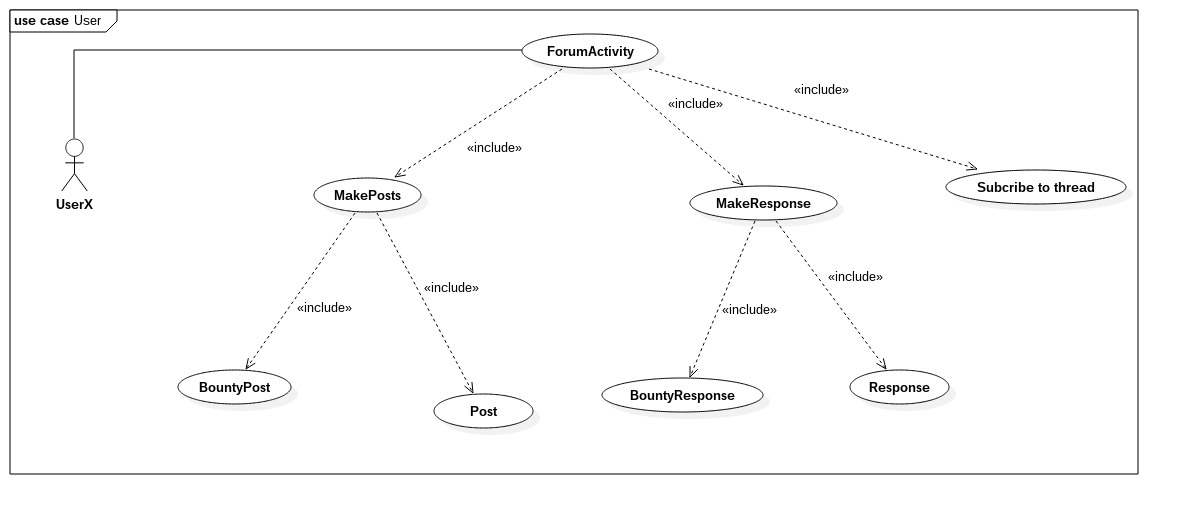
\includegraphics[width=\linewidth]{Diagrams/ForumActivityUC.jpg}
\caption{Scope of the Users Module.}
\end{figure}

\subsubsection{Domain model}
\par{The domain model for the user module is represented in the figure below, there are two types of users: a student user and a user of elevated privilege/reputation. Users with higher reputation range from Teaching Assistants to Lecturers and course coordinators. The stock user is able to build up their reputation on the platform, the details for this are left to the discussion on the Gamification module.}

\begin{figure}[h!]
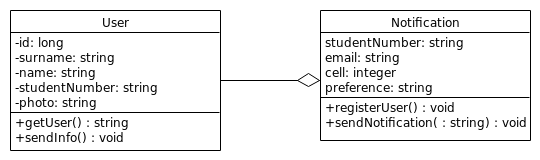
\includegraphics[width=\linewidth]{Diagrams/userDomain.png}
\caption{User domain model.}
\end{figure}

\par{}

\subsubsection{Use cases}
\subsubsection*{Login (AuthN)}
\par{This will be a functionality that authenticates each users, through managing and controlling access to the system, by requesting the user to enter their credentials. A session will be created for the user after a successful login. Figure 4 describes the process of login and authentication of a user by the platform using LDAP.}

\bigskip
\par{\textbf{Precondition:} The user is a authenticated on LDAP.}
\par{\textbf{Exception:} If user is not authenticated, return an empty User Object.}
\par{\textbf {Postcondition:} No change}
\par{\textbf {Return:} a User Object with user details. }

\begin{figure}[h!]
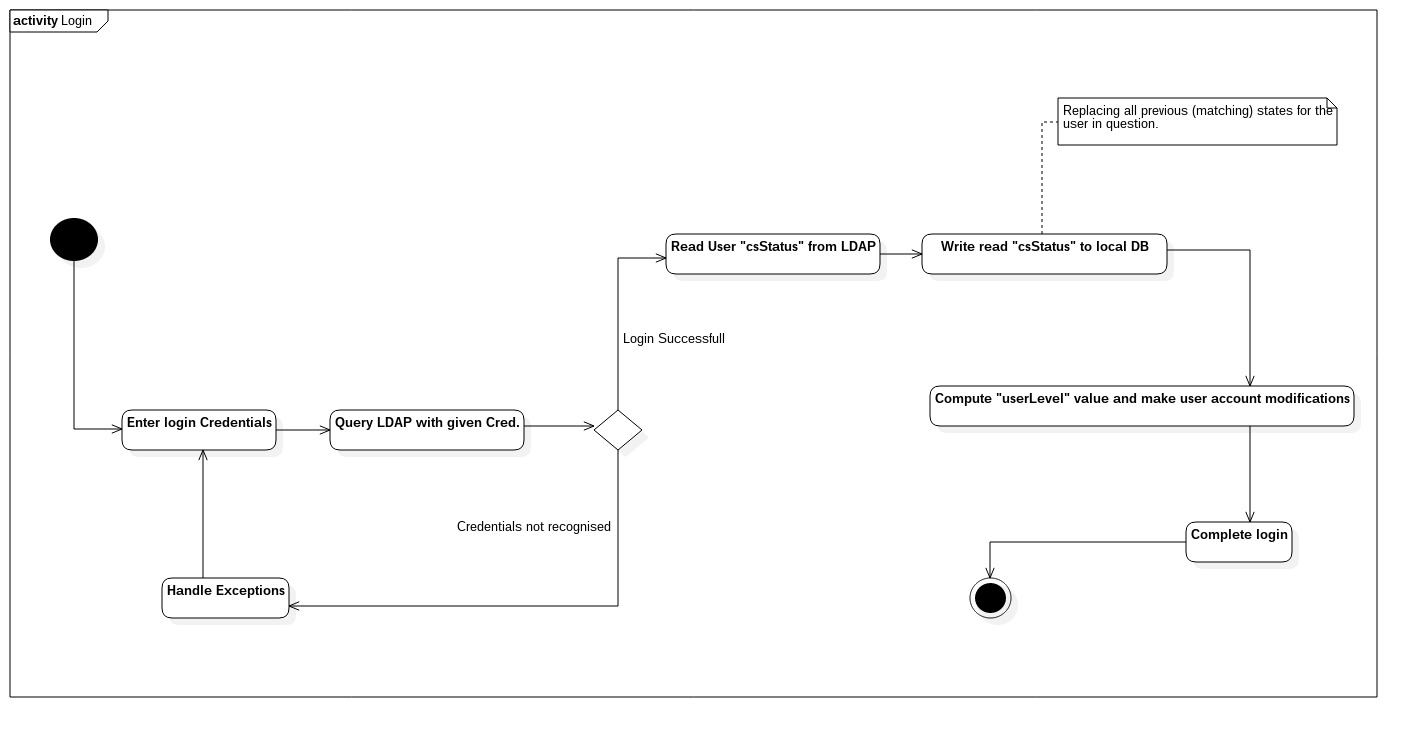
\includegraphics[width=\linewidth]{Diagrams/BuzzLoginAct.jpg}
\caption{Login/AuthN Sequence diagram.}
\label{Use-case: Authentication}
\end{figure}

\subsubsection*{Get user information}
\par{This will be the functionality that allows lectures to retrieve the information of a specific user within the system. Only users who are enrolled in the module which the lecture presents will be returned.}

\subsubsection{Security}
\par{Role based access control has been applied to restrict system access to authorized users. Users of the system have different roles within the system, which are then assigned different permissions.}
\smallskip
\par{The primary rules of Role-Based Access Control as applied in the system.}
\begin{enumerate} 
	\item Role assignment: 
    \begin{itemize}
      \item Students have been assigned permission to access the forum modules, within the system, which they are enrolled to.
      \item Admin users have been assigned permission to access the forum modules, within the system, which they present.
      \end{itemize}
      \item Role authorization: 
    \begin{itemize}
      \item Student authorization is done by verifying their status on LDAP, which is then validated through their status defined on the system’s database.
      \item Admin user authorization is done by verifying the lectures credentials on LDAP, then retrieving all the modules which they present. 
 	\end{itemize}
	\item Permission authorization: 
    \begin{itemize}
    \item Once validated, students have access to forum modules which they have been verified to use. Making them unable to access modules they are not enrolled in. 
	\item As admin users, lectures have permission to access to the student’s information, for the module which they present
    \end{itemize}
\end{enumerate}

\smallskip
\par{A table to describe the design of the role based access control.}
\begin{center}
	\begin{tabu} to 1.2\textwidth{ | X[l] | X[c] | X[r] | }
    	\hline
        	\textbf{Subject:} & Student & Higher level User \\
        \hline 
         	\textbf{Role:} & Low level user & Admin \\
        \hline 
          	 \textbf{Resources:} & \begin{itemize}
                                     \item{Posts}
                                     \item{Reports}
                                     \item{Group}
                                     \item{User profile}
                                   \end{itemize} 
                                 & \begin {itemize} 
									  \item{Posts}
                                      \item{User profile}
                                      \item{Reports}
                                      \item{Audit log}
                                    \end{itemize} \\
        \hline
        	\textbf{Operations:} & \begin {itemize}
  								     \item{Create and Read posts}
                                     \item{View reports of user contribution}
                                     \item{Create and Delete groups}
                                     \item{Edit user profile details}
                                   \end{itemize}
           						 & \begin{itemize} 
                                 	\item{Create, Read, Update and Delete posts}
                                    \item{View profiles of users enrolled in their module}
                                    \item{Generate reports of user activity within the forum module, for statistical analysis.}
                                    \item{Generate an audit log to view and maintain users activity within the system.}
                                  \end{itemize} \\
        \hline 
    \end{tabu}   
\end{center}

\smallskip

\par{User credentials, userID and password, are encrypted using RSA encryption during transmission and are decrypted during the query to LDAP. User information retrieved from LDAP is then encrypted before transmission back to the system and then decrypted before being stored on the systems database.User passwords are not stored within the systems database, users are authorized through LDAP for access to the system. }

\newpage
\subsection*{User level names}
\par{Below is a description of the kinds of users the forum should have, to add an element of gamification to the user CS-Status module a user will be assigned a user-status name which will indicate the user-level of the user (CS-Status). These user-status names should be as follows: }
\begin{itemize}
\item Variable: All stock-users (students) are assigned the user-level-name "variable" by default.
\item Function: All tutors are assigned the user-level-name "function" by default.
\item Class: All Tutorial-Assistants are assigned the user-level-name "class" by default.
\item Library: All Lectures are assigned the user-level-name "library" by default.
\end{itemize}

\paragraph*{}{Note: a user will have a user-level-name for each of the course modules they are registered for that are supported by the forum. Meaning that a user can be a "variable" in one module and a "class" in another module. A unique colour will be associated with each user-level-name enabling the user status of a user to be quickly distinguishable.}



\newpage
\subsection{CS-Status Module}
\par{Each user on the forum has a user status termed CS-Status. A users status (CS-Status) is determined by the role(s) he/she plays in one or more course modules. Thus from a persons CS-Status we are able to filter out what privileges the person should have on the forum and for which course modules.}
\subsubsection{Scope}
\par{The CS-Status of a user will be used for authorization purposes on the forum. Users of higher statuses will be able to perform additional actions on the forum that stock-users will not be able to perform.}
\subsubsection{Use cases}
\subsubsection*{Create CS Status}
\par{Upon login, the users CS-Status will be queried from LDAP and the local copy of the state of the user will be overwritten (for safety and efficiency). This ensures that any changes that may have taken place (updates to the users state) are persisted to our local databases.}
\subsubsection*{Get Status Symbol}
\par{When the user information is fetched from LDAP, the state of the user (for each of their course modules) must be transfered to an instance of the CS-Status module.}
\subsubsection{Domain model}
\par{The figure of the CS-Status domain model is in figure ~\ref{fig:cs}.}
\begin{figure}[h!]
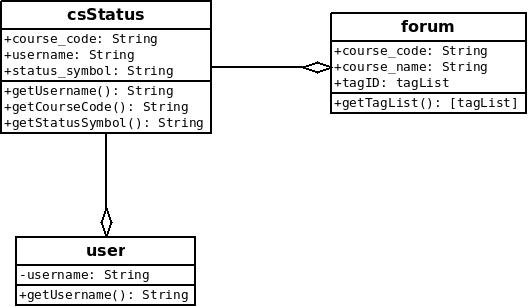
\includegraphics[width=\linewidth]{Diagrams/csStatus_domain_model.jpeg}
\caption{Domain model representing the CS status model}
\label{fig:cs}
\end{figure}


\newpage
\subsection{Post Module}
\par{The post model will be a service used to post messages to the forum. The messages will be in the form of either posts and comments.}
\subsubsection{Requirements}
\subsubsection*{Functional}
\begin{itemize}
\item Handle the posting and accessing of forum content as well as structuring forum threads in an orderly manner.
\item Three types of posts can be made. The creation of a thread (level-zero post), the response to a post and the creation of a bounty post. 
\end{itemize}

\subsection*{Types of posts}
\begin{itemize}
\item {Level-zero post: The first post for a specified topic is termed a level-zero post. A topic will only have one level-zero post which can be seen as a the root in a hierarchy of related posts}
\item {Child-post: Responses to posts are termed child-posts. Child posts become parent posts to other posts when responses are made to that child post.}
\item {Sibling-Post: Posts at the same level within the same topic are termed sibling posts.}
\item {Bounty-post: Users are able to make posts in the form of questions with an attached reward to be awarded to the person who gives a correct answer to this question. We call such a post a bounty-post. This feature forms part of the gamification module and will be further more discussed in the Gamification module.}
\end{itemize}

\subsubsection{Use cases}
\subsubsection*{Create Post}
\par{This will be a functionality which will allow users to create new posts for the course module they belong to. If they are adding on to an already existing post then it will fall under that post. The posts structure will follow a tree structure. Upon creating a post, tags will also be created that accompany that post.}
\subsubsection*{Edit Post}
\par{This will be a service for users with higher privileges. It will allow them to edit various posts. The main edits will be on tags of a post.}
\subsubsection*{Remove Post}
\par{This will be a service for users with higher privileges. It will allow them to remove various posts, meaning that they will no longer be visible to other users. When a post is removed, all the posts and comments that accompany and fall under it will also be removed.}
\subsubsection{Domain Model}
\begin{itemize}
\item A new post will be on level 0, making its heading the name of the thread.
\item The level of a new post, under another post, will be an increment of the post that it falls under.
\item A post cannot be created by a user who does not belong to the module. 
\end{itemize}
\begin{figure}[h!]
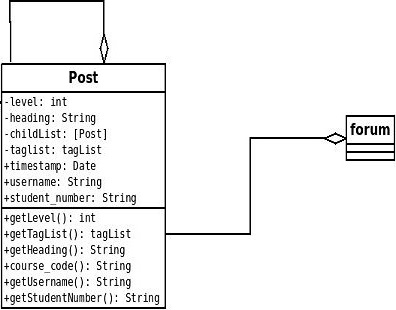
\includegraphics{Diagrams/posts_domain_model.jpeg}
\caption{Domain model representing the message model}
\label{fig:mesg}
\end{figure}

\newpage
\subsection{Notifications Module}
\par{This module will be responsible for the handling of User notifications.}
\subsubsection{Scope}
\par{Users will have the option of subscribing to Forum content and receiving notifications on this specific content via email.}

%\begin{figure}[h!]
%\includegraphics[width=\linewidth]{}
%\caption{Scope of the Buzz-Notification Module.}
%\end{figure}

\subsubsection{Use cases}
\subsubsection*{Add notification}
\par {The user will be able to make additions to the list of content he/she wants notifications on. This will be handled in the form of subscriptions.}
\subsubsection*{Remove notification}
\par{This involves the removal of subscriptions when a user does not want to receive anymore notifications on the said content or posts.}

\subsubsection{Service Contracts}
\par{The notification requests will need to be of a specific type and properly validated before being processed. The request will fail if it does not meet its specified prerequisites. In order for a notification request to be passed on to the server, the user needs to already exist on the database. If this requirement is not met, a notification request will fail. Once a user has subscribed to receive notification on a said topic the following will be accomplished:}
\medskip
\begin{itemize}
\item Notify user of new posts for the subscribed thread.
\item Notify user of new responses made for the subscribed thread.
\item Notify user of new bounty-posts made for the subscribed thread.
\end{itemize}

\subsubsection{Technologies}
\begin{itemize}
\item The linking of the notification with the thread or post it is associated with will be done using JavaScript.This will allow for dynamic posting of notifications, without the administrator having to manually create every notification.
\item Google Email is an API with a capacity to service a number of email within a limit. The API will be ideal to provide messaging capacity for the system without having to implement email servers internally.
\end{itemize}

\subsubsection{Domain Model}
\par{The domain model for the notifications module is represented in figure 6 below:}

\begin{figure}[h!]
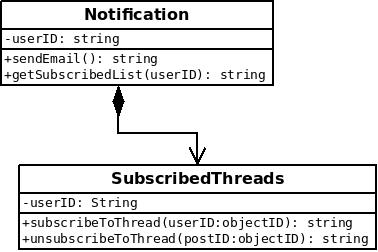
\includegraphics[width=\linewidth]{Diagrams/NotificationDM.jpeg}
\caption{Domain model of Notifications}
\end{figure}

\begin{figure}[h!]
%\includegraphics[width=\linewidth]{}
\caption{Domain model of Notifications}
\end{figure}
\newpage

\subsection{Reports Module}
\par{The Reports module is used to provide statistical information that can be used by the lecture to observe overall usage of the forum and award rewards to users that participate constructively to the forum. Management can also use the data collected to make updates and maintain the system. The statistics module can be separated into the following layers:}

\subsection*{Personal Statistics}
\par{All users are able to view their own statistics and also stats related to the course modules they are participating in.}
\subsection*{User Statistics}
\par{Admin users will be able to view the statistics of individual users. These stats include the number of posts, likes, dislikes and overall participation.}
\subsection*{Course statistics}
\par{Admin users will be able to view statistics for a specified course module. These stats include the activity within a said period of time (ie: a week or month).}
\subsection*{Forum statistics}
\par{The statistics relating to overall forum activity is meant more for the platform administrators than the course module admin.}

\subsubsection{Use cases}
\par{The reporting module provides services to gather statistical information for each user and export a report back to the lecture, who can assess the user’s overall usage of the forum.}

\subsection*{getTotalPosts}
\par{The system will store the assessed user profile to generate a total for the number of posts a user has made. This statistical information will be saved and exported to the lecture/management.}
\subsection*{ComputeAverages}
\par{An effective way to present statistics is by representing them as averages over a given sample size. Factors like averagePostsPerWeek will be represented by averages across a collection of users for the said course module.}

\subsubsection{Domain Model}
\begin{figure}[h]
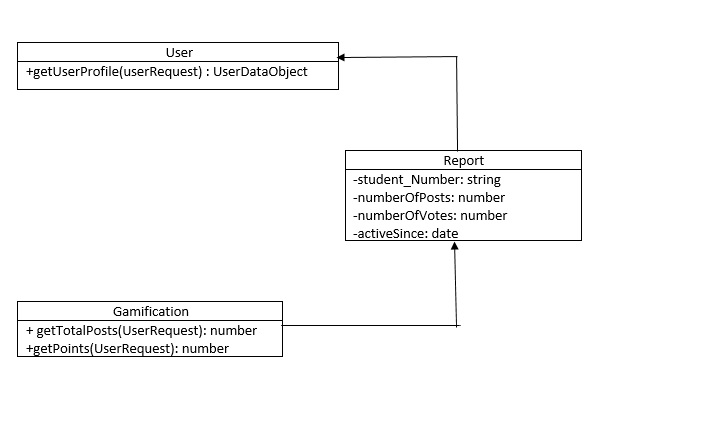
\includegraphics[width=\linewidth]
{Diagrams/report_domain_model.jpeg}
\caption {Domain model of the Buzz-Report module.}
\end{figure}


\newpage
\subsection{Authorization Module (AuthZ)}
\par{This module will be used to authorize a user, therefore allowing or denying a user from performing a specified task or operation within the forum.
}

\subsubsection{Scope}
\par{As explained, the forum will have different types of users and each user will be limited as to what operations they can perform within the forum. Upon requesting to perform the specified operation, a user will be verified as authorized or notAuthorized by this module. }

\subsubsection{Use cases}
\subsection*{authorizeUser}
\par{Check that a user is authorized to perform a specified operation. If user is successfully authorized the operation is triggered, else the operation is not performed. The criteria used to determine whether a user is allowed to perform a said operation is the user-level of the user which is dependent on the users forum status. However, with the use of gamification and the rewards system, a user is able to climb up the ranks and achieve the ability to perform non-stock operations.} 

\subsection{Gamification Module}
\par{This module will be used to add another dimension to the discussion chat platform by including a gamifying factor which will help make the system as a whole interactive as one can measure their progress, not only does it make it exciting but also promotes participation.}
\subsubsection{Scope}
\par{This module will be the backbone of the gamification attribute to the system, to which the administrator has the ability to change/assign titles as well as bounty requirements.}

\begin{figure}[h!]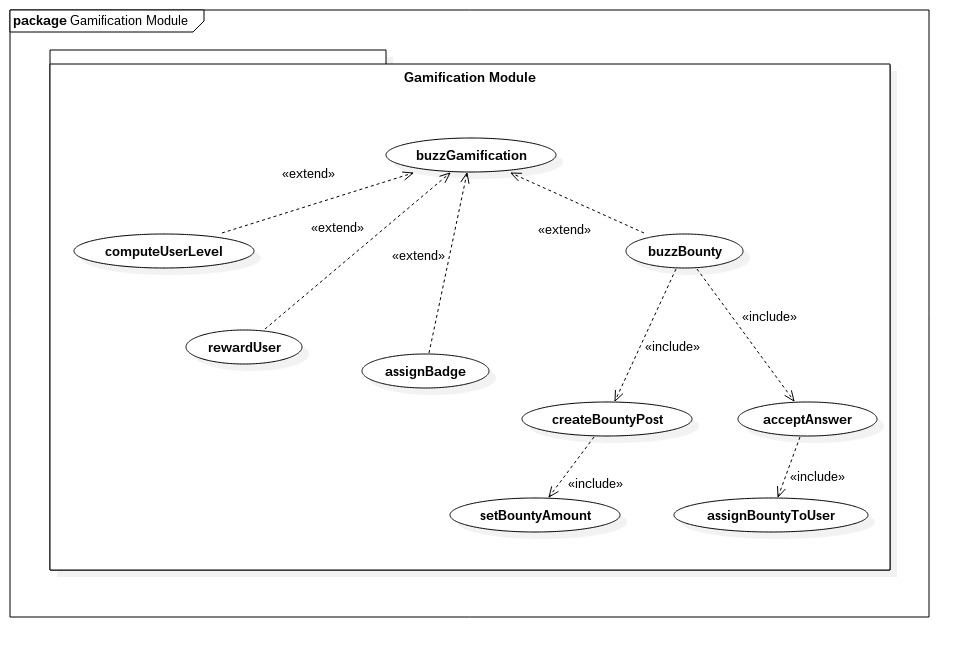
\includegraphics[width=\linewidth]{Diagrams/buzzGami.jpg}
\caption{Scope of the Gamification Module.}
\label{Use-case: Gamification}
\end{figure}
\subsubsection{Use Cases}
\subsubsection*{Status promotion}
\par{This is in the event that a user's status is to be promoted.}
\subsubsection*{Status demotion}
\par{This is in the event that a user's status is to be demoted.}
\subsubsection*{Increase bounty}
\par{This is in the event that a user has done something to have their points increase.}
\subsubsection*{Decrease bounty}
\par{This is in the event that something has occurred that must decrease the bounty points of the user.}
\subsubsection*{Create Group}
\par{This pertains to the event of a new group being created by a user.}
\subsubsection*{Assign titles}
\par{This is an administrative feature that enables the administrator to further adjust aspects of the game.}

\subsubsection{Service Contracts}
\subsubsection*{Calculate Status}
\par{This is used to determine what is the current status of a user, using a formula that is based on the current level their currently on}
\subsubsection*{Status promotion}
\par{A person is given a new status due to them accumulating enough points to deserve a promotion, after their status is calculated.}
\subsubsection*{Status demotion}
\par{A person is given a prior status, after their status is calculated, due to them loosing enough points to deserve a demotion.}
\subsubsection*{Increase bounty}
\par{A person has their bounty points increased due to them performing a positive act of participation on the site, such as posting, or having another user do something in relation to their action such as like their post.}
\subsubsection*{Create Group}
\par{This is the event in which someone spends their currency to create a group, to which other members are able to join in and interact on their on private exclusive thread.}
\subsubsection*{Assign titles}
\par{The administrator is able to set the name and number of different titles (levels) the users can obtain as well the number of points required to achieve each.}


\subsubsection{Domain Model}
\begin{figure}[h!]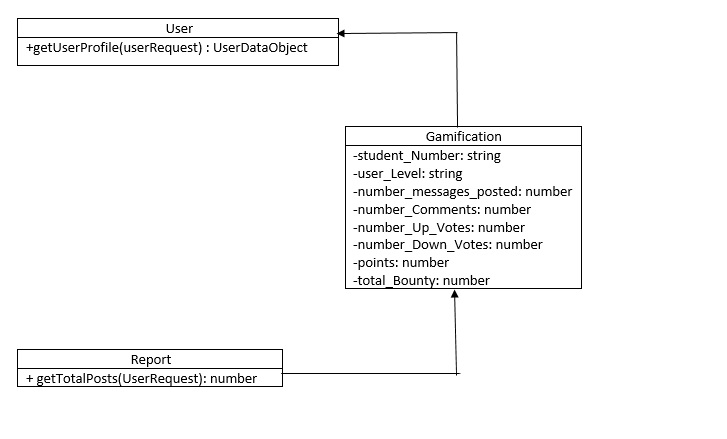
\includegraphics[width=\linewidth]{Diagrams/gamificationDomainModel.jpeg}
\caption{Domain model of the Gamification module.}
\end{figure}
\newpage


\subsection{Subscriptions Module}
\par{The Subscriptions module handles content subscriptions made by the user. These subscriptions include subscriptions to level-zero posts. }
\subsubsection{Scope}
\par{The scope of the Subscriptions Module is modeled by Figure 25. Users have the option of subscribing to particular Posts or topics. The User will then have the option to receive Notifications via email on the content of their subscriptions.}

\begin{figure}[h!]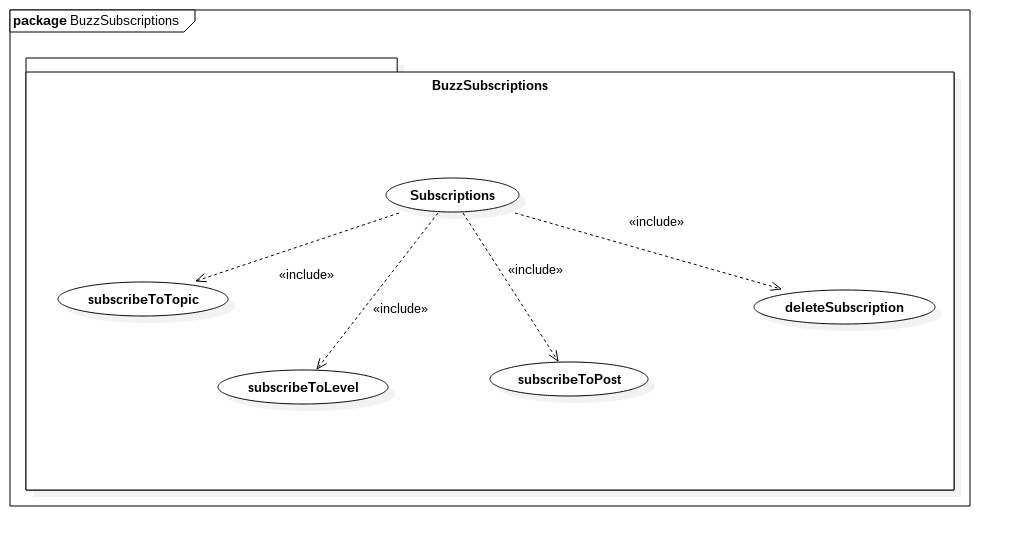
\includegraphics[width=\linewidth]{Diagrams/buzzSubscriptions.jpg}
\caption{Scope of the Subscriptions Module.}
\label{Use-case: Subscriptions}
\end{figure}

\subsubsection{Use Cases}
\subsubsection*{Subscribe to topic}
\par{User will be notified on all content for a specified topic within a Forum-Module. This includes all created child posts into infinity.}
\subsubsection*{Subscribe to level}
\par{User will be notified on only the activity for a given post and its immediate child posts.}
\subsubsection*{Subscribe to post}
\par{User will be notified on all activity related to this post and all its child post.}
\subsubsection*{Delete subscription}
\par{Removal of a subscription to a users subscription list. Resulting in the user not receiving notifications on the topic or post in the future.}

\subsubsection{Service Contracts}
\subsubsection*{Subscriptions}
\par{A user can only subscribe to a topic or post to which they have registered for in the current academic term.}
\subsubsection*{Notifications}
\par{A user has the option of specifying to which email account notifications should be sent to.}

\newpage
\section{Glossary}
\begin{itemize}
\item {\textbf{Software Architecture} -  Structured solution that meets all of the technical and operational requirements of the system.}
\item {\textbf{Service oriented software} -  Style of software design where services are provided to the other components by application components, through a communication protocol over a network.}
\item{\textbf{Coupling} - a measure of how closely connected two routines or modules are.}
\item {\textbf{Model-View Controller} - Software architectural pattern for implementing user interfaces on computers by dividing a given application into three interconnected parts.}
\item{\textbf{RSA encryption} - A  public key cryptography algorithm used in the encrypting and decrypting of messages.}
\item{\textbf{DB-Schema} - Database Schema is a structure used to describe the organization of data within the database.}
\item{\textbf{csStatus} - The role of the user for a specific module i.e. lecture, student, tutor}
\item{\textbf{Netiquette} - The correct or acceptable way of communicating on the Internet. }
\item{\textbf{Level-Zero post} - The first post created in a topic for a specified module. }
\item{\textbf{Child post} - A reply to a post.}
\item{\textbf{Sibling post} - Posts on the same level are called siblings. Thus posts with the same parent are termed siblings.}
\item{\textbf{Parent post} - See level-zero post. }
\item{\textbf{Forum-Module} - A module/subject that is registered on the forum and is presented by the institution in question.}
\item{\textbf{Forum-Module} - A module/subject that is registered on the forum and is presented by the institution in question.}
\item{\textbf{LDAP} - "(Lightweight Directory Access Protocol) is a software protocol for enabling anyone to locate organizations, individuals, and other resources such as files and devices in a network, whether on the public Internet or on a corporate intranet." - Wikipedia}
\item{\textbf{Stock user} - a basic user with no added privileges on the forum. A stock user can only perform the basic operations on the forum.}
\item{\textbf{AuthN} - The process of verifying that a user is "who they say they are" after this user has identified themself.}
\item{\textbf{AuthZ} - The process of verifying that a said user has the right to access system assets/ objects or perform certain operations within the platform/system.}
\end{itemize}

\end{document}
